\chapter{Context Survey}
\section{Context}
\subsection{History}

In the early 2000s, the University of St.\ Andrews' School of Computer Science had a class size of approximately 30 students. It has had a relatively rapid expansion in recent years, with class size of over 200 students. Although the student to staff ratio in manned computer laboratory sessions has remained fairly consistent throughout the years, the logistics of class management became more difficult. This increasing difficulty has been increasing educators awareness of the need for an alternative solution.

As lockdown measures were introduced in the wake of the global pandemic, the University was forced to move to online learning and the need for an alternative to in-person labs became immediate. Completely remote online teaching is a novel experience for the University, presenting many challenges. The School developed a system for managing online labs using Microsoft Teams \cite{teams}, adapting it in an ad hoc manner to improve the flow and features by integrating with additional systems such as Sharepoint Lists \cite{lists}, Forms \cite{forms} and Power Automate \cite{pauto}. The current system meets the basic needs for managing online labs, however, it lacks more sophisticated lab management facilities, such as gathering statistical data as well as searching and recommending solutions to posted problems.   

The School of Computer Science requires a system for managing labs that meets its specific needs. The system should be suitable for in-person, remote and dual delivery. It should enable class demonstrators to assist in the resolution of problems students have, should enable lab leads to review labs and address some of the specific nuances that the domain requires - for example addressing the lab opening times. A single application should meet these needs so that the system is easy to use, adapt and maintain.

There are some existing categories of application which could meet the above needs. A small number of classroom management tools exist in the form of queue management systems. Another, much more common, type of application are incident management tools - often used for tracking and logging IT incidents and problems. Both types of application shall be considered and evaluated in order to gain insight into their suitability.
 
This chapter shall discuss and review two common examples of these types of application, as well as the current system used by the school.

\subsection{Online Learning}

TODO read ruth suggested papers and include

As the world becomes more online as a result of the global pandemic \cite{bbcinternet} \cite{ofcominternet}, careful consideration should be given to the techniques and systems used to teach and study online. Consideration of this research and review of its conclusions could prove invaluable in identifying the most critical parts of an online lab management system. This short subsection shall discuss some key discoveries from a literature review in this area.

The system used by University members will have a direct affect on their satisfaction with both working and studying from home \cite{tenney}. Although the system will also be used to facilitate in-person labs, we should carefully consider the aspects of the system useful for home working since the system is more critical in facilitating online labs than in-person labs. 

Satisfaction and a positive attitude toward work increases the likelihood that students will achieve higher productivity levels \cite{tenney}. The perceived usefulness of the tools that students have access to while \gls{wfh} will also affect productivity \cite{venka}. Student satisfaction and attitude will be directly affected by the tools and system that they use to interact with the University online which will, in turn, increase their ability to work productively \cite{safaa}. This points directly to the design of a bespoke system, which will be the most directly useful and also appear the most visibly useful to users.

Another important aspect of online learning is students' perceived feeling of support. One of the most importants roles of an online instructor is students feeling their `presence’ \cite{martinteams}. `Being there’ for students and `having a presence that the students felt on the course site’ is essential \cite{martin}. For this reason, the system which is used to manage labs should strive to maximise students' awareness of the demonstrators who are available to help them. 

\section{Current System}

The current system for managing online lab sessions was developed and adapted at short notice due to the global pandemic. The initial solution was to create a `CS1000 Labs' team on Microsoft Teams \cite{teams}, the University's standard collaboration tool for online learning, and manage the lab sessions by posting announcements when labs opened. Students were then able to post new conversations under these announcements, with instructions to tag the class demonstrators, in which they briefly summarised their issue and provided the module code and practical number associated with their issue (see Figure \ref{fig:firstit}).

There were a few problems with this system. As the numbers of posts in the channel increased, it became more difficult to find the `next' person who should get help. This problem was exacerbated by the algorithm that Teams uses to order posts, which was not appropriate or intuitive for the lab channel. Demonstrators were instructed to use the `Activities' tab in Teams that maintained the correct order, however this did not help resolve the difficulty in finding the `next' request. For some of the busier lab sessions, related to practical deadlines, additional, non-regular demonstrators were brought in to help. These demonstrators did not have access to the activities history and therefore had to revert to using the non-ordered main Teams channel.

\FloatBarrier
\begin{figure}[H]
  \centering
  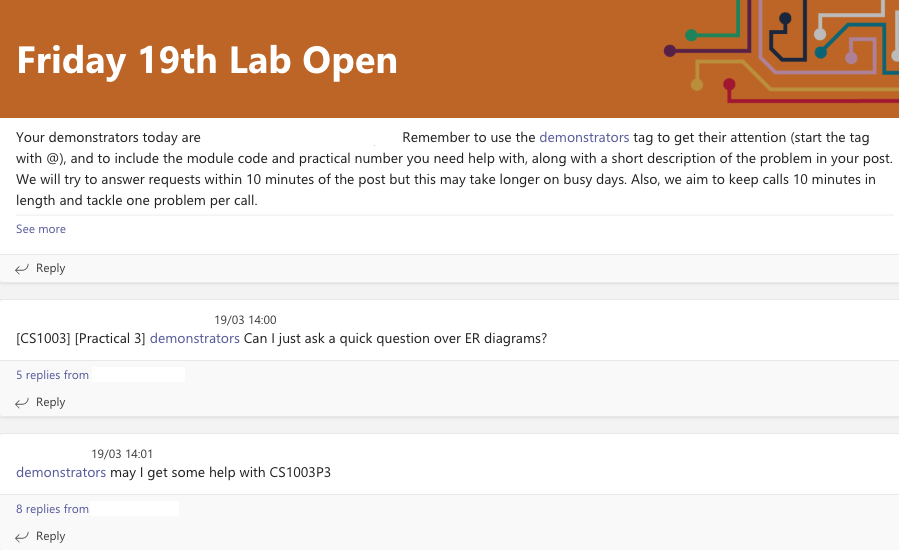
\includegraphics[width=\textwidth]{2context/images/teams1.png}
  \label{fig:firstit}
  \caption{An example of the first iteration process of managing online labs.}
\end{figure}

The second iteration of the system was created by using a Power Automate Flow to create an entry in a Sharepoint List when students posted an issue request to the channel. Class demonstrators used the list to show the chronological order of requests, see which demonstrator was handling each request and to mark requests as resolved. This intermediate iteration addressed most of the major issues from the first iteration, however had its own problems. There could be a delay of up to 15 minutes between the student posting in the teams channel and the request appearing on the Sharepoint List. This delay would be forgiveable in the busier labs, however is clearly unacceptable for the first 15 minutes of labs or for days on which there were less requests.

The third, and current, iteration of the current system uses a form input (see Figure \ref{fig:form}). This is accessed using a `Request Form' tab in the Microsoft Teams \cite{teams} CS1000 Labs team. 

\FloatBarrier
\begin{figure}[H]
  \centering
  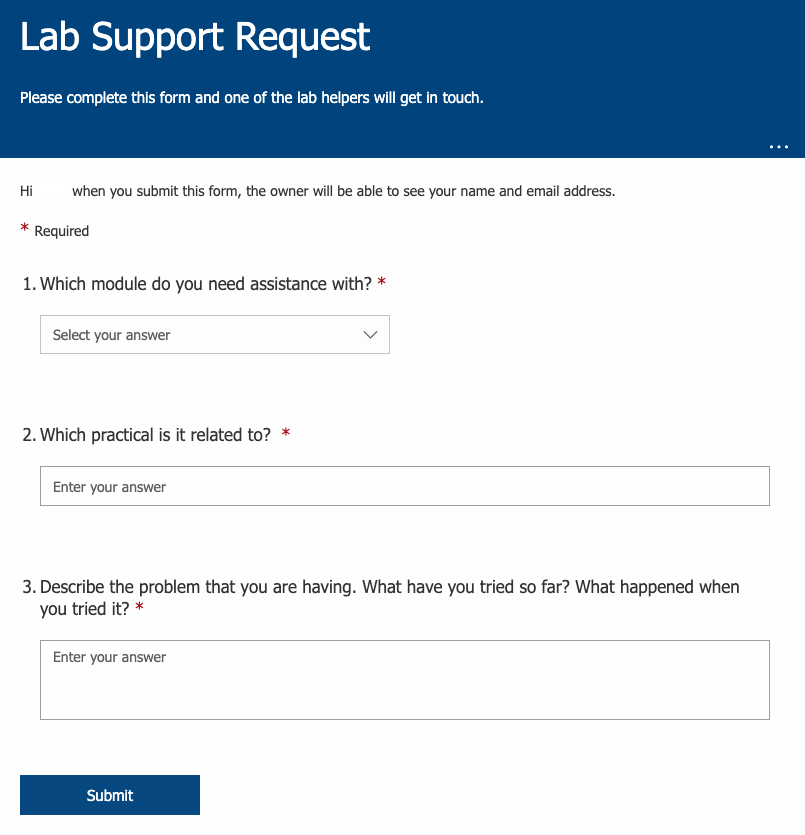
\includegraphics[width=0.85\textwidth]{2context/images/teams2a.png}
    \label{fig:form}
  \caption{The request form from the second iteration process of managing online labs.}
\end{figure}

The form uses Power Automate \cite{pauto} to post (see Figure \ref{fig:privteam}) on a private demonstrator team channel (used only to create a notification for class demonstrators) and add the form data to a Microsoft List \cite{lists}.

\FloatBarrier
\begin{figure}[H]
  \centering
  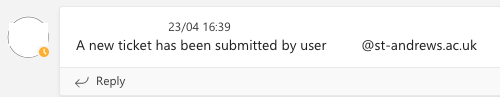
\includegraphics[width=0.6\textwidth]{2context/images/teams2b.png}
  \caption{The format of posts on the private demonstrator channel used to create notifications.}
  \abel{fig:privteam}
\end{figure}

On this real-time collaborative form, class demonstrators can assign themselves to students' requests before they make contact with the student through Microsoft Teams \cite{teams}. The lab lead would also contact students by email if their request was missed, because there were too many requests to deal with during the time that class demonstrators were hired, or if the request was made outside of manned lab hours. The activity diagram below (see Figure \ref{fig:activdiagram}) shows the workflow for the current system during an open lab.

\FloatBarrier
\begin{figure}[H]
  \centering
  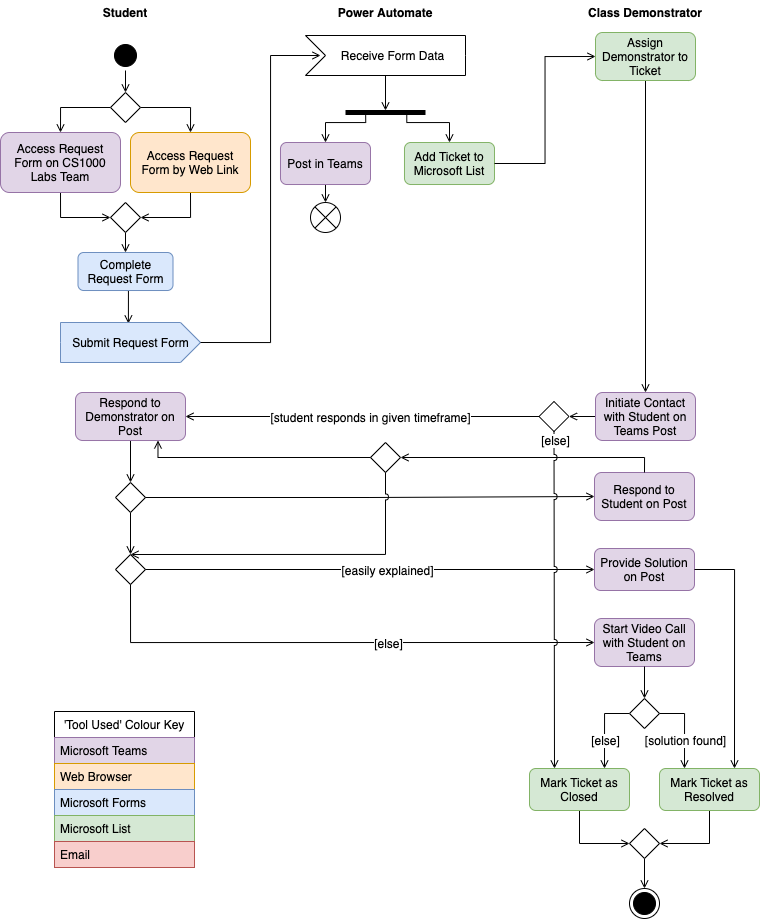
\includegraphics[width=\textwidth]{2context/images/activityRevised.png}
  \caption{\gls{uml} Activity diagram for existing method of managing student online lab request when lab is open.}
  \label{fig:activdiagram}
\end{figure}

\newpage
\section{Queue Management Tools}

Queue management tools are tools that all you to sign-in, be assigned a place in a queue and get a notification when you have reached the head of the queue. They can be be used for accessing a digital or physical resource.

ClassroomQ is a good example of existing queue management tool, applying a queue management tool to an educational context. It offers a very simple system, where a teacher can create a classroom which students can join, type a message and hit an `Assistance Needed' button to join the queue of students who need help. The basic process is shown below.

Firstly, the teachers start a classroom session (see Figure \ref{fig:cqstart}).

\FloatBarrier
\begin{figure}[H]
  \centering
  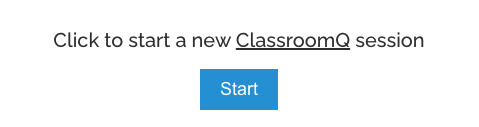
\includegraphics[width=0.5\textwidth]{2context/images/cq1.png}
  \caption{Teacher's screen when a class has not been started.}
  \label{fig:cqstart}
\end{figure}

The classroom is created, showing the class code which students can use to join (see Figure \ref{fig:cqstart}).

\FloatBarrier
\begin{figure}[H]
  \centering
  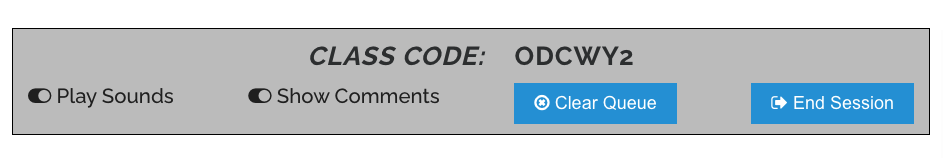
\includegraphics[width=0.75\textwidth]{2context/images/cq2.png}
  \caption{Real time classroom queue, showing class join code and current requests.}
  \label{fig:cqcode}
\end{figure}

Students join by entering their name and class code (see Figure \ref{fig:cqjoin}).

\FloatBarrier
\begin{figure}[H]
  \centering
  
\includegraphics[width=0.5\textwidth]{2context/images/cq3.png}
  \caption{Student join page, showing sample class code and name.}
  \label{fig:cqjoin}
\end{figure}

One students have joined the class, they are able to input details of their problem in the comment section and then click the `Assistance Needed' button to join the queue (see Figure \ref{fig:cqbutton}).

\FloatBarrier
\begin{figure}[H]
  \centering
  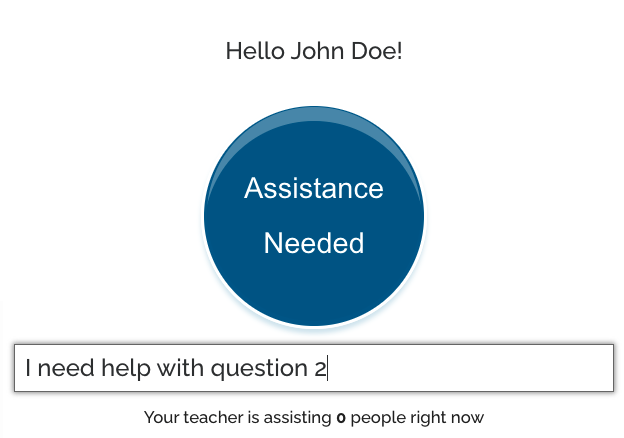
\includegraphics[width=0.5\textwidth]{2context/images/cq4.png}
  \caption{Student help request page.}
  \label{fig:cqbutton}
\end{figure}

Once the student has joined the queue, they are shown a page which allows them to cancel their request whilst showing real time information about their position in the queue (see Figure \ref{fig:cqbutton2}).

\FloatBarrier
\begin{figure}[H]
  \centering
  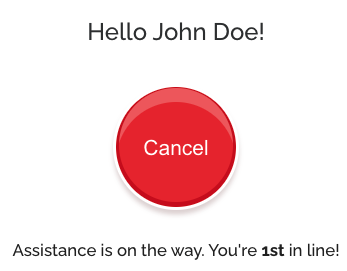
\includegraphics[width=0.5\textwidth]{2context/images/cq5.png}
  \caption{Student page after posting help request.}
  \label{fig:cqbutton2}
\end{figure}

The teacher is then able to see an ordered view of the student's requests in on the class page (see Figure \ref{fig:cqclass}).

\FloatBarrier
\begin{figure}[H]
  \centering
  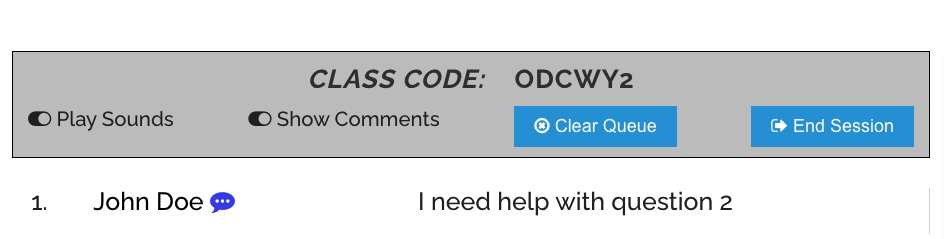
\includegraphics[width=0.75\textwidth]{2context/images/cq6.png}
  \caption{Teacher's class page view after the request has been posted.}
  \label{fig:cqclass}
\end{figure}

\newpage
\section{Incident Management Tools}

Incident management tools are used by IT professionals to organise, categorise and prioritise issue tickets as well as to track their resolution. These incidents can be posted by the IT professionals themselves or by other third parties who are reporting them. These tools, compared with queue management tools, offer significantly more in terms of power of automation, configurability and feature sets. However, these benefits come at the price of greater overheads in setup and maintenance.

Spiceworks Cloud Help Desk is a good example of existing incident management tools. It is a free to use, cloud-based help desk that is used by IT professionals. Traditionally, the system is used to track and manage IT issues in order to provide IT support, however the system could also be used to track and manage requests for help in our lab management domain. In the following section we shall discuss the basic process workflow of using Spiceworks to manage students' ticket requests.

TODO Ruth: 'This is all a bit speculative - I would prefer a discussion of the general incident management process followed by a brief discussion of how the lab management problem could fit into this.'

Firstly, students would access a link to the help portal and enter their email address (see Figure \ref{fig:spiceemail}).

\FloatBarrier
\begin{figure}[H]
  \centering
  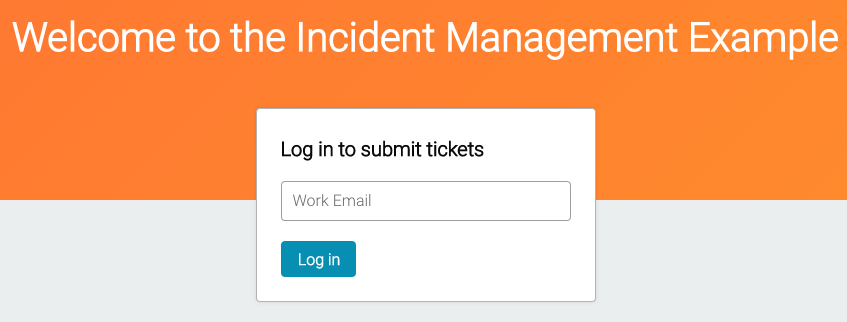
\includegraphics[width=0.5\textwidth]{2context/images/SWportalLogin.png}
  \caption{Login screen from portal link.}
  \label{fig:spiceemail}
\end{figure}

The student would then, if authorised, receive an email link to login to the portal. This would take them to a form in which they would describe their issue (see Figure \ref{fig:spiceform}).

\FloatBarrier
\begin{figure}[H]
  \centering
  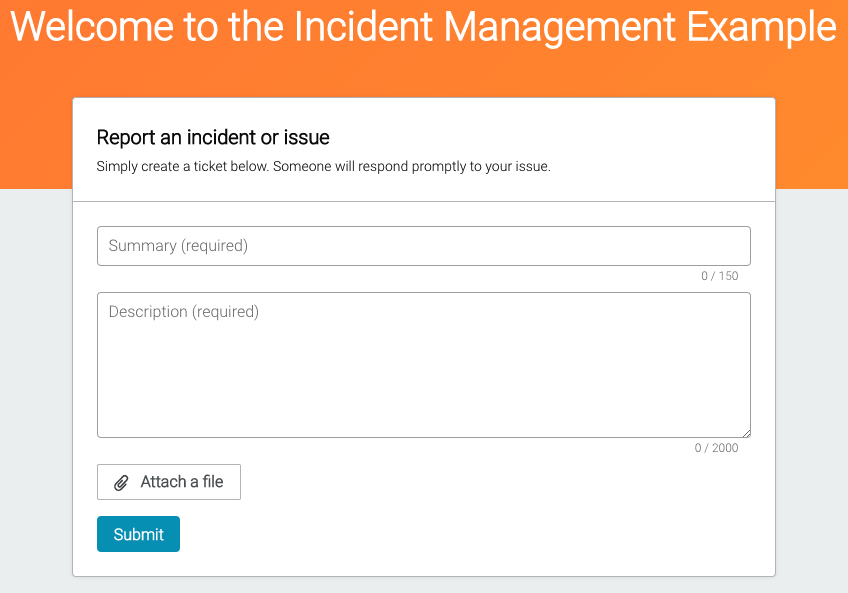
\includegraphics[width=0.65\textwidth]{2context/images/SWpostTicket.png}
  \caption{Ticket posting form, reached after login.}
  \label{fig:spiceform}
\end{figure}

The ticket would then appear on the class demonstrator help desk (see Figure \ref{fig:spicedesk}).

\FloatBarrier
\begin{figure}[H]
  \centering
  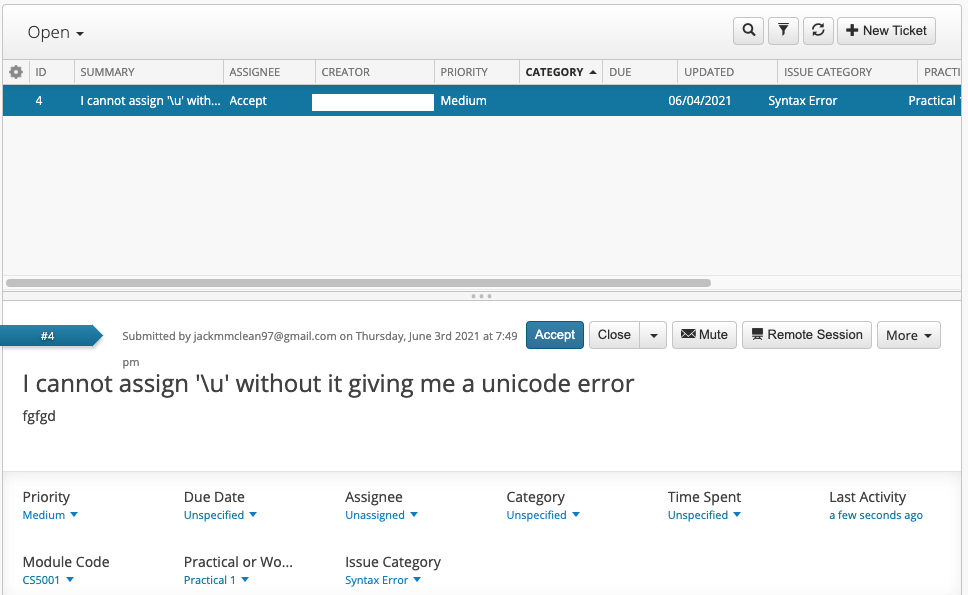
\includegraphics[width=0.85\textwidth]{2context/images/SWticketPage.png}
  \caption{The help desk ticket page, accessible to class demonstrators.}
  \label{fig:spicedesk}
\end{figure}

Class demonstrators are then able to respond to the ticket on Spiceworks, notifying the user by email, and initiate a video call on a different service if necessary. The demonstrator can then close the ticket when complete.

